\documentclass[journal,12pt,twocolumn]{IEEEtran}

\usepackage{setspace}
\usepackage{gensymb}

\singlespacing


\usepackage[cmex10]{amsmath}

\usepackage{amsthm}

\usepackage{mathrsfs}
\usepackage{txfonts}
\usepackage{stfloats}
\usepackage{bm}
\usepackage{cite}
\usepackage{cases}
\usepackage{subfig}

\usepackage{longtable}
\usepackage{multirow}

\usepackage{enumitem}
\usepackage{mathtools}
\usepackage{steinmetz}
\usepackage{tikz}
\usepackage{circuitikz}
\usepackage{verbatim}
\usepackage{tfrupee}
\usepackage[breaklinks=true]{hyperref}
\usepackage{graphicx}
\usepackage{tkz-euclide}
\usepackage{float}

\usetikzlibrary{calc,math}
\usepackage{listings}
    \usepackage{color}                                            %%
    \usepackage{array}                                            %%
    \usepackage{longtable}                                        %%
    \usepackage{calc}                                             %%
    \usepackage{multirow}                                         %%
    \usepackage{hhline}                                           %%
    \usepackage{ifthen}                                           %%
    \usepackage{lscape}     
\usepackage{multicol}
\usepackage{chngcntr}

\DeclareMathOperator*{\Res}{Res}

\renewcommand\thesection{\arabic{section}}
\renewcommand\thesubsection{\thesection.\arabic{subsection}}
\renewcommand\thesubsubsection{\thesubsection.\arabic{subsubsection}}

\renewcommand\thesectiondis{\arabic{section}}
\renewcommand\thesubsectiondis{\thesectiondis.\arabic{subsection}}
\renewcommand\thesubsubsectiondis{\thesubsectiondis.\arabic{subsubsection}}


\hyphenation{op-tical net-works semi-conduc-tor}
\def\inputGnumericTable{}                                 %%

\lstset{
%language=C,
frame=single, 
breaklines=true,
columns=fullflexible
}
\begin{document}
\newtheorem{theorem}{Theorem}[section]
\newtheorem{problem}{Problem}
\newtheorem{proposition}{Proposition}[section]
\newtheorem{lemma}{Lemma}[section]
\newtheorem{corollary}[theorem]{Corollary}
\newtheorem{example}{Example}[section]
\newtheorem{definition}[problem]{Definition}

\newcommand{\BEQA}{\begin{eqnarray}}
\newcommand{\EEQA}{\end{eqnarray}}
\newcommand{\define}{\stackrel{\triangle}{=}}
\bibliographystyle{IEEEtran}
\providecommand{\mbf}{\mathbf}
\providecommand{\pr}[1]{\ensuremath{\Pr\left(#1\right)}}
\providecommand{\qfunc}[1]{\ensuremath{Q\left(#1\right)}}
\providecommand{\sbrak}[1]{\ensuremath{{}\left[#1\right]}}
\providecommand{\lsbrak}[1]{\ensuremath{{}\left[#1\right.}}
\providecommand{\rsbrak}[1]{\ensuremath{{}\left.#1\right]}}
\providecommand{\brak}[1]{\ensuremath{\left(#1\right)}}
\providecommand{\lbrak}[1]{\ensuremath{\left(#1\right.}}
\providecommand{\rbrak}[1]{\ensuremath{\left.#1\right)}}
\providecommand{\cbrak}[1]{\ensuremath{\left\{#1\right\}}}
\providecommand{\lcbrak}[1]{\ensuremath{\left\{#1\right.}}
\providecommand{\rcbrak}[1]{\ensuremath{\left.#1\right\}}}
\theoremstyle{remark}
\newtheorem{rem}{Remark}
\newcommand{\sgn}{\mathop{\mathrm{sgn}}}
\providecommand{\abs}[1]{\vert#1\vert}
\providecommand{\res}[1]{\Res\displaylimits_{#1}} 
\providecommand{\norm}[1]{\lVert#1\rVert}
%\providecommand{\norm}[1]{\lVert#1\rVert}
\providecommand{\mtx}[1]{\mathbf{#1}}
\providecommand{\mean}[1]{E[ #1 ]}
\providecommand{\fourier}{\overset{\mathcal{F}}{ \rightleftharpoons}}
%\providecommand{\hilbert}{\overset{\mathcal{H}}{ \rightleftharpoons}}
\providecommand{\system}{\overset{\mathcal{H}}{ \longleftrightarrow}}
	%\newcommand{\solution}[2]{\textbf{Solution:}{#1}}
\newcommand{\solution}{\noindent \textbf{Solution: }}
\newcommand{\cosec}{\,\text{cosec}\,}
\providecommand{\dec}[2]{\ensuremath{\overset{#1}{\underset{#2}{\gtrless}}}}
\newcommand{\myvec}[1]{\ensuremath{\begin{pmatrix}#1\end{pmatrix}}}
\newcommand{\mydet}[1]{\ensuremath{\begin{vmatrix}#1\end{vmatrix}}}
\numberwithin{equation}{subsection}
\makeatletter
\@addtoreset{figure}{problem}
\makeatother
\let\StandardTheFigure\thefigure
\let\vec\mathbf
\renewcommand{\thefigure}{\theproblem}
\def\putbox#1#2#3{\makebox[0in][l]{\makebox[#1][l]{}\raisebox{\baselineskip}[0in][0in]{\raisebox{#2}[0in][0in]{#3}}}}
     \def\rightbox#1{\makebox[0in][r]{#1}}
     \def\centbox#1{\makebox[0in]{#1}}
     \def\topbox#1{\raisebox{-\baselineskip}[0in][0in]{#1}}
     \def\midbox#1{\raisebox{-0.5\baselineskip}[0in][0in]{#1}}
\vspace{3cm}
\title{GATE ASSIGNMENT 2}
\author{MANIKANTA VALLEPU \\ AI20BTECH11014}
\maketitle
\newpage
\bigskip
\renewcommand{\thefigure}{\theenumi}
\renewcommand{\thetable}{\theenumi}
Download all python codes from 
\begin{lstlisting}
https://github.com/AI20BTECH11014/EE3900-Linear-Systems-and-Signal-processing/blob/main/Gate_Assignment_2/GATE_Assignment_2.py
\end{lstlisting}
%
and latex-tikz codes from 
%
\begin{lstlisting}
https://github.com/AI20BTECH11014/EE3900-Linear-Systems-and-Signal-processing/blob/main/Gate_Assignment_2/Gate_Assignment_2.tex
\end{lstlisting}
%
\section{EC 2007 Q.16}
If the Laplace transform of a signal $y\brak{t}$ is $$y\brak{s}=\dfrac{1}{s(s-1)}$$then its final value is 
\begin{enumerate}
    \item -1
    \item 0
    \item 1
    \item unbounded
\end{enumerate}
\section{Solution}
\begin{theorem}
FINAL VALUE THEOREM
\text{The final value theorem states}
\begin{align}
   	\lim_{t \to +\infty} f\brak{t} = \lim_{s \to 0} sF\brak{s}
\end{align}
It determines the steady-state value of the system response without finding the inverse transform.It is applicable only for stable systems.
\end{theorem}
Given,
$$y\brak{s}=\dfrac{1}{s(s-1)}$$
from Final value theorem,
\begin{align}
   	\lim_{t \to +\infty} y\brak{t} &= \lim_{s \to 0} sy\brak{s}\\
   	&= \lim_{s \to 0} s\dfrac{1}{s(s-1)}\\
   	&= \lim_{s \to 0} \dfrac{1}{(s-1)}
\end{align}
s=1 is right s-plane pole of $y\brak{s}$ with ROC $\abs{s}>1$ .As the system is not lining left half of s-plane,the system is unstable.Hence, it is unbounded.
$\therefore$ option 4 is correct.
\begin{figure}[!h]
 \centering
 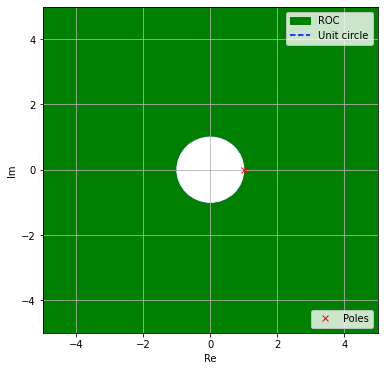
\includegraphics[width=\columnwidth]{fig_GA_1.png}
 \caption{ROC for $y\brak{s}$.}
\end{figure}
\begin{lemma}[Table of Inverse Laplace Transforms]\label{tbl}
\begin{center}
\begin{tabular}{ |m{3cm}|m{4.5cm}| } 
 \hline
 $\textbf{Laplace transform}$ of f(t) $F\brak{s}=\mathcal{L}\cbrak{f\brak{t}}$  & $\textbf{Time Function}$$ f(t)=\mathcal{L}^{-1}\cbrak{F(s)}$ \\ 
 \hline
 $\dfrac{1}{s}$, $s>0$ &1 \\ 
 \hline
 $\dfrac{1}{s-a}$, $s-a>0$ & $e^{at}$\\
 \hline
\end{tabular}
\end{center}
\end{lemma}

\begin{lemma}{Linearity of Inverse Laplace Transform} \label{l2}
\begin{align}
    \mathcal{L}^{-1}\cbrak{af\brak{t}+bg\brak{t}}=a\mathcal{L}^{-1}\cbrak{f\brak{t}}+b\mathcal{L}^{-1}\cbrak{g\brak{t}}
\end{align}
\end{lemma}

\begin{align}
    y\brak{t}&= \mathcal{L}^{-1}\cbrak{y\brak{s}}\\
    &= \mathcal{L}^{-1}\cbrak{\dfrac{1}{s(s-1)}}\\
     &= \mathcal{L}^{-1}\cbrak{\dfrac{-1}{s} + \dfrac{1}{s-1}}
\end{align}
From Lemma-\ref{l2},
\begin{align}
    &= \mathcal{L}^{-1}\cbrak{\dfrac{-1}{s}} +  \mathcal{L}^{-1}\cbrak{
    \dfrac{1}{s-1}}
\end{align}
From Lemma-\ref{tbl},
\begin{align}
     y\brak{t}&= -1 + e^{t}
\end{align}
\begin{figure}[!h]
 \centering
 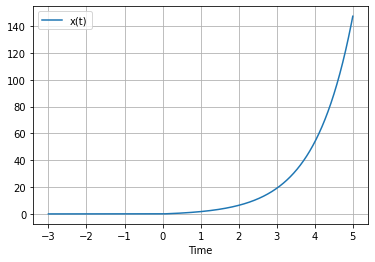
\includegraphics[width=\columnwidth]{fig_2.png}
 \caption{plot of $y\brak{t}$ in input domain.}
\end{figure}
\end{document}
